\documentclass[tikz, border=5pt]{standalone}% 'crop' is the default for v1.0, before it was 'preview'
\usepackage{tikz}
\usepackage{pgfplots}
\usepackage{amsmath}

% \usepgfplotslibrary{colormaps}
\pgfplotsset{compat=1.18}
\usetikzlibrary{plotmarks, arrows.meta, shapes, calc}
%\usetikzlibrary{...}% tikz package already loaded by 'tikz' option
\begin{document}


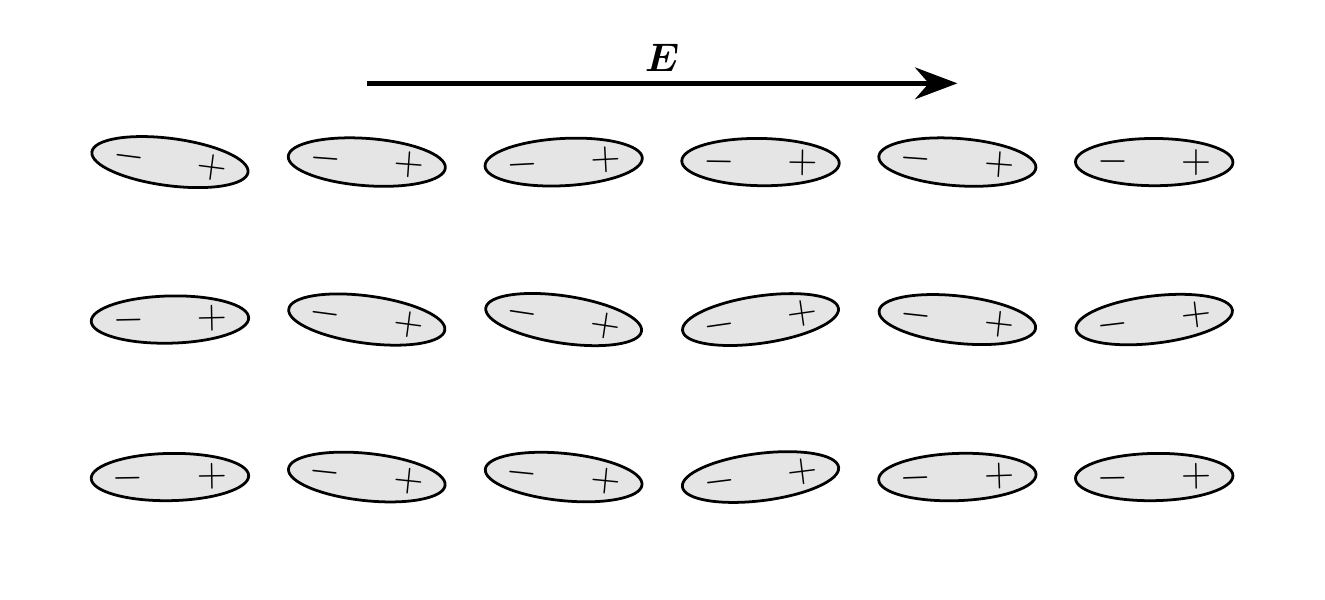
\begin{tikzpicture}[font=\Large]
  % Define a pic that takes two arguments:
  %   #1 = centre coordinate, e.g. (0,0)
  %   #2 = rotation angle in degrees, e.g. 30
  \tikzset{
    pics/rotated-ellipse/.style n args={2}{
      code={
        \begin{scope}[rotate around={#2:#1}, transform shape]
          % Hard-coded ellipse geometry
          \draw[fill=gray!20, line width=1pt]
            #1 ellipse [x radius=1cm, y radius=0.3cm];

          % Labels, placed along the major axis before rotation
          \node[anchor=east, font=\Large] at ($#1 + ( 0.85, 0)$) {$+$};
          \node[anchor=west,  font=\Large] at ($#1 + (-0.85, 0)$) {$-$};
        \end{scope}
      }
    }
  }

  \foreach \cx/\cy/\ang in {
    0/0/1.0,
    2.5/0/-6.0,
    5/0/-5.7,
    7.5/0/7.1,
    10/0/2.0,
    12.5/0/1.0,
    0/2/1.3,
    2.5/2/-7.6,
    5/2/-8.5,
    7.5/2/8.2,
    10/2/-6.3,
    12.5/2/6.8,
    0/4/-7.4,
    2.5/4/-4.2,
    5/4/3.0,
    7.5/4/-0.9,
    10/4/-4.1,
    12.5/4/-0.1
  }{
    \pic {rotated-ellipse={(\cx,\cy)}{\ang}};
  }

  \draw[ultra thick, -{Stealth[scale=1.5]}]
    (2.5,5) -- (10,5)
    node[midway, above] {$\boldsymbol{E}$};

  \draw[white] (-1.8, -1.2) rectangle (14.3, 5.7); 
\end{tikzpicture}
\end{document}